\documentclass{beamer}
\usepackage[utf8]{inputenc}
\usetheme{default}
\usecolortheme{dove}
\usepackage{textpos}
\usepackage{grid-system}
\usepackage[official]{eurosym}


% po4a: environment frame
% po4a: environment Row
% po4a: environment Cell


\title{Freifunk Darmstadt}
\author{
\includegraphics[width=4cm]{images/logo}}
%\institute[Inst.]{Freifunk Darmstadt}
\date{29. Januar 2014}

\begin{document}

\begin{frame}
\maketitle
\end{frame}

\addtobeamertemplate{frametitle}{}{%
\begin{textblock*}{100mm}(0.93\textwidth,-0.5cm)

\includegraphics[height=1cm]{images/logo}
\end{textblock*}}

\begin{frame}{Outline}
\tableofcontents
\end{frame}

\section{Einleitung}
\begin{frame}{Freifunk in Deutschland}
\vfill
\begin{center}
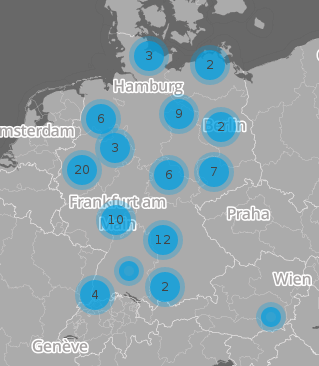
\includegraphics[height=0.6\textheight]{images/map}$\;$
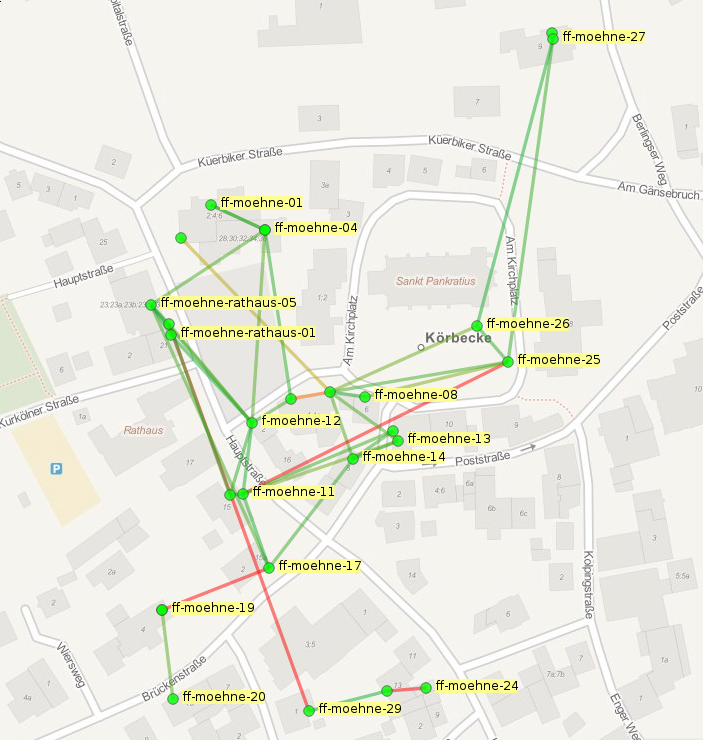
\includegraphics[height=0.6\textheight]{images/moehne}
\end{center}
\vfill
\end{frame}

\section{Projektbeschreibung}
\begin{frame}{Projektbeschreibung}
\vfill
\begin{center}
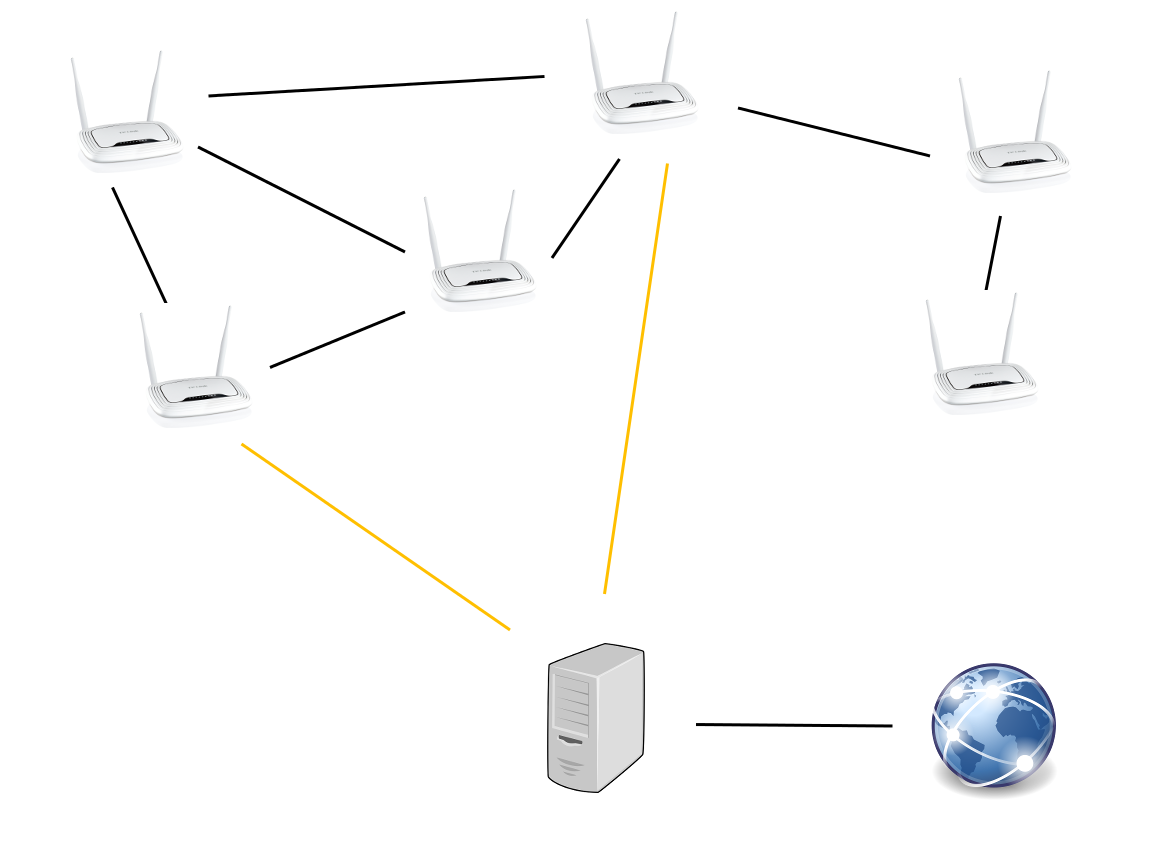
\includegraphics[height=0.7\textheight]{images/meshing}
\end{center}
\vfill
\end{frame}

\section{Aktueller Stand}
\begin{frame}{Aktueller Stand}
\vfill
\begin{center}
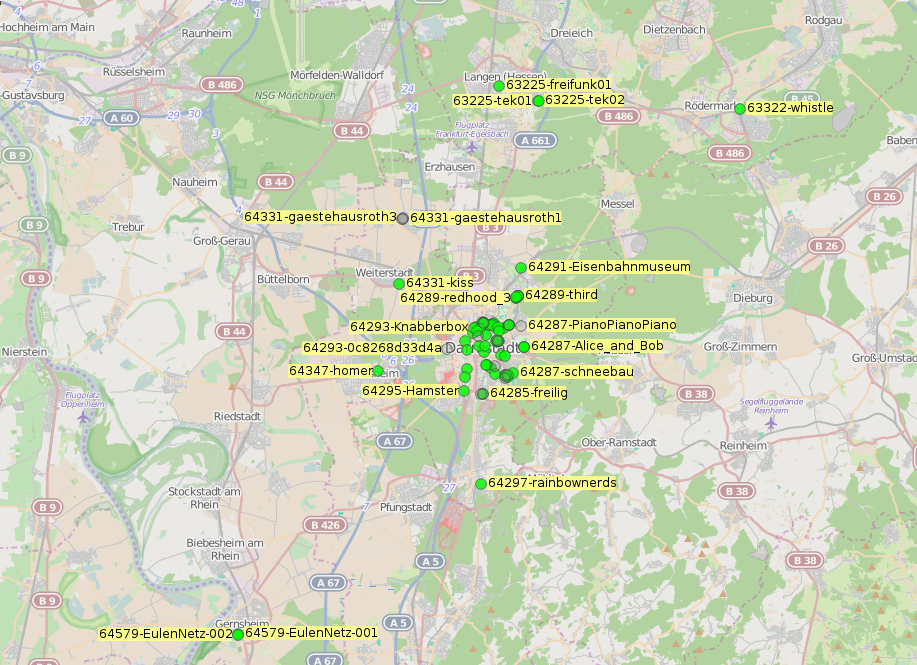
\includegraphics[height=0.75\textheight]{images/2015-01-26-map}$\;$
\vfill
ca. 80 Accesspoints
\end{center}
\end{frame}

\begin{frame}{Aktueller Stand - Darmstadt}
\vfill
\begin{center}
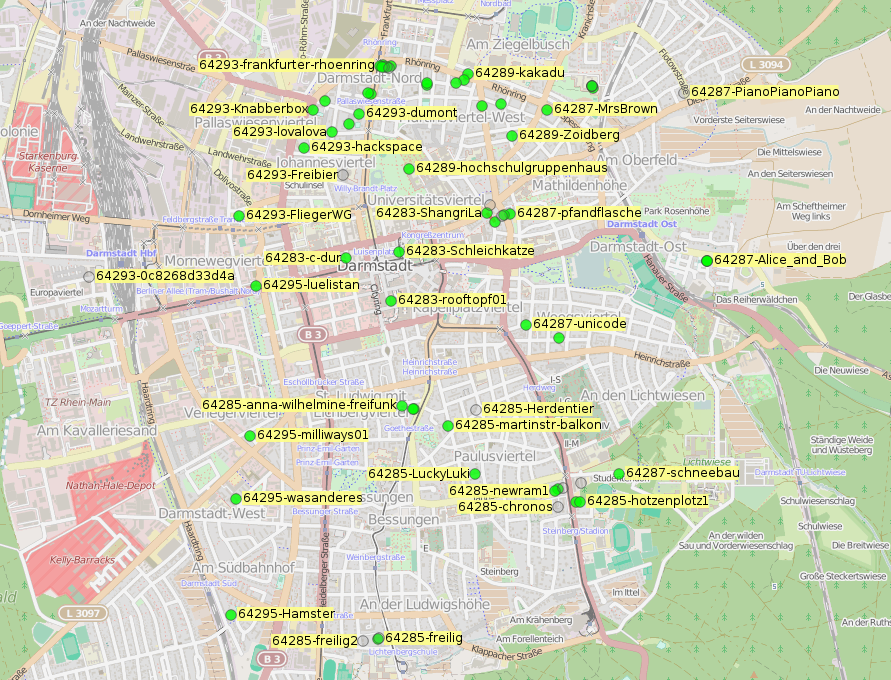
\includegraphics[height=0.75\textheight]{images/2015-01-26-darmstadt}$\;$
\vfill
\end{center}
\end{frame}

\begin{frame}{Aktueller Stand - K6}
\vfill
\begin{center}
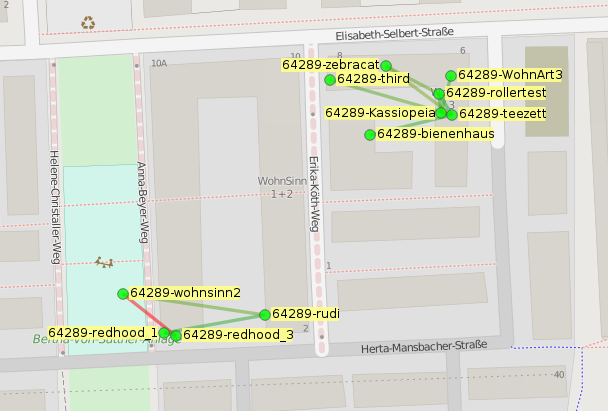
\includegraphics[height=0.75\textheight]{images/2015-01-26-wohnart3}$\;$
\vfill
\end{center}
\end{frame}

\section{Ausbauplan}
\begin{frame}{Ausbauplan}
\vfill
\begin{itemize}
	\item öffentliche Plätze und Staatstheater, Haltestellen, Krankenhäuser, \ldots)
	\item Hotels, Gaststätten, öffentliche Einrichtungen, \ldots
	\item Parks (z.B. Herrengarten, Prinz-Emil-Garten, \ldots)
	\item private Wohnungen, Studentenwohnheime, \ldots
	\item hochgelegene Plätze für Richtfunk (Langer Ludwig, Kirchtürme, Hochzeitsturm, h$\_$da Hochhaus \ldots)
\end{itemize}
\vfill
\begin{itemize}
	\item zur Abdeckung stellen private oder öffentliche Anlieger der Freifunk-Community Standorte zur Verfügung oder betreiben eigene Freifunk-Router
	\item Durchführung von Informationsveranstaltungen und Workshops zur Steigerung des Bekanntheitsgrades
\end{itemize}
\vfill
\end{frame}

\section{Verwendete Router-Hardware}
\begin{frame}{Verwendete Router-Hardware}
Handelsübliche Modelle im 2.4GHz- und 5GHz-Band
\vfill
Für den Heimbedarf oder kleinere öffentliche Bereiche:
\begin{itemize}
\item bis zu 20 Clients pro Gerät
\item 30-50\euro{}
\end{itemize}
\vfill

Größere Inneninstallationen:
\begin{itemize}
\item bis zu 200 Clients pro Gerät
\item ca. 250\euro{}
\end{itemize}
\vfill

Außeneinsatz:
\begin{itemize}
\item bis zu 200 Clients pro Gerät
\item Kosten abhängig von Frequenzband, Geschwindigkeit und Antennentyp, 100-600\euro{}
\end{itemize}
\vfill
\end{frame}

\section{Beispiel Luisenplatz}
\begin{frame}{Beispiel: Luisenplatz}
Wie sieht die Leistungsfähigkeit der technischen Lösung am Beispiel Luisenplatz aus?
\end{frame}

\section{Anforderungen an die Stadt}
\begin{frame}{Anforderungen an die Stadt}
\vfill
\begin{center}
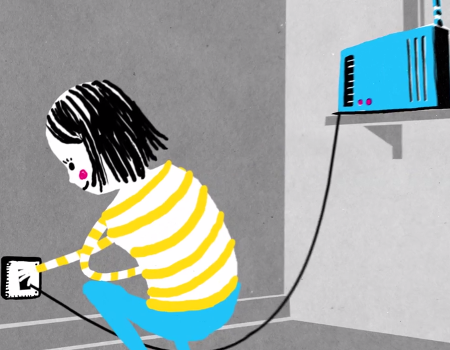
\includegraphics[height=0.4\textheight]{images/setup}$\;$
\vfill
\end{center}
\begin{itemize}
\item Bereitstellung von Standorten/Montageflächen
\item Bereitstellung von Strom und Internetanbindung/Richtfunk
\item Kauf oder Sponsoring der notwendigen Hardware
\item evtl. Durchführung professioneller Montagearbeiten
\end{itemize}
\vfill
\end{frame}

\section{Betrieb}
\begin{frame}{Betrieb}
Wie wird der Betrieb sichergestellt?
Ist ein durchgehender Betrieb sichergestellt?
Welche Reaktionszeiten/Wiederherstellungszeiten werden garantiert?
\vfill
We do not operate the devices. We only provide the firmware and VPN infrastructure and can be consulted w.r.t. coverage issues and other problems.
\end{frame}


\end{document}
